\label{sec:cnninterrupt}
% The idea of interruption is introduced for dynamic multi-task scheduling. This section details the implementation of our \textbf{Virtual instruction Interruption}. \Cref{fig:interDPR} illustrates the idea of interruption to full utilize the hardware resources.


% \begin{figure*}[t]
% 	\centering
% 	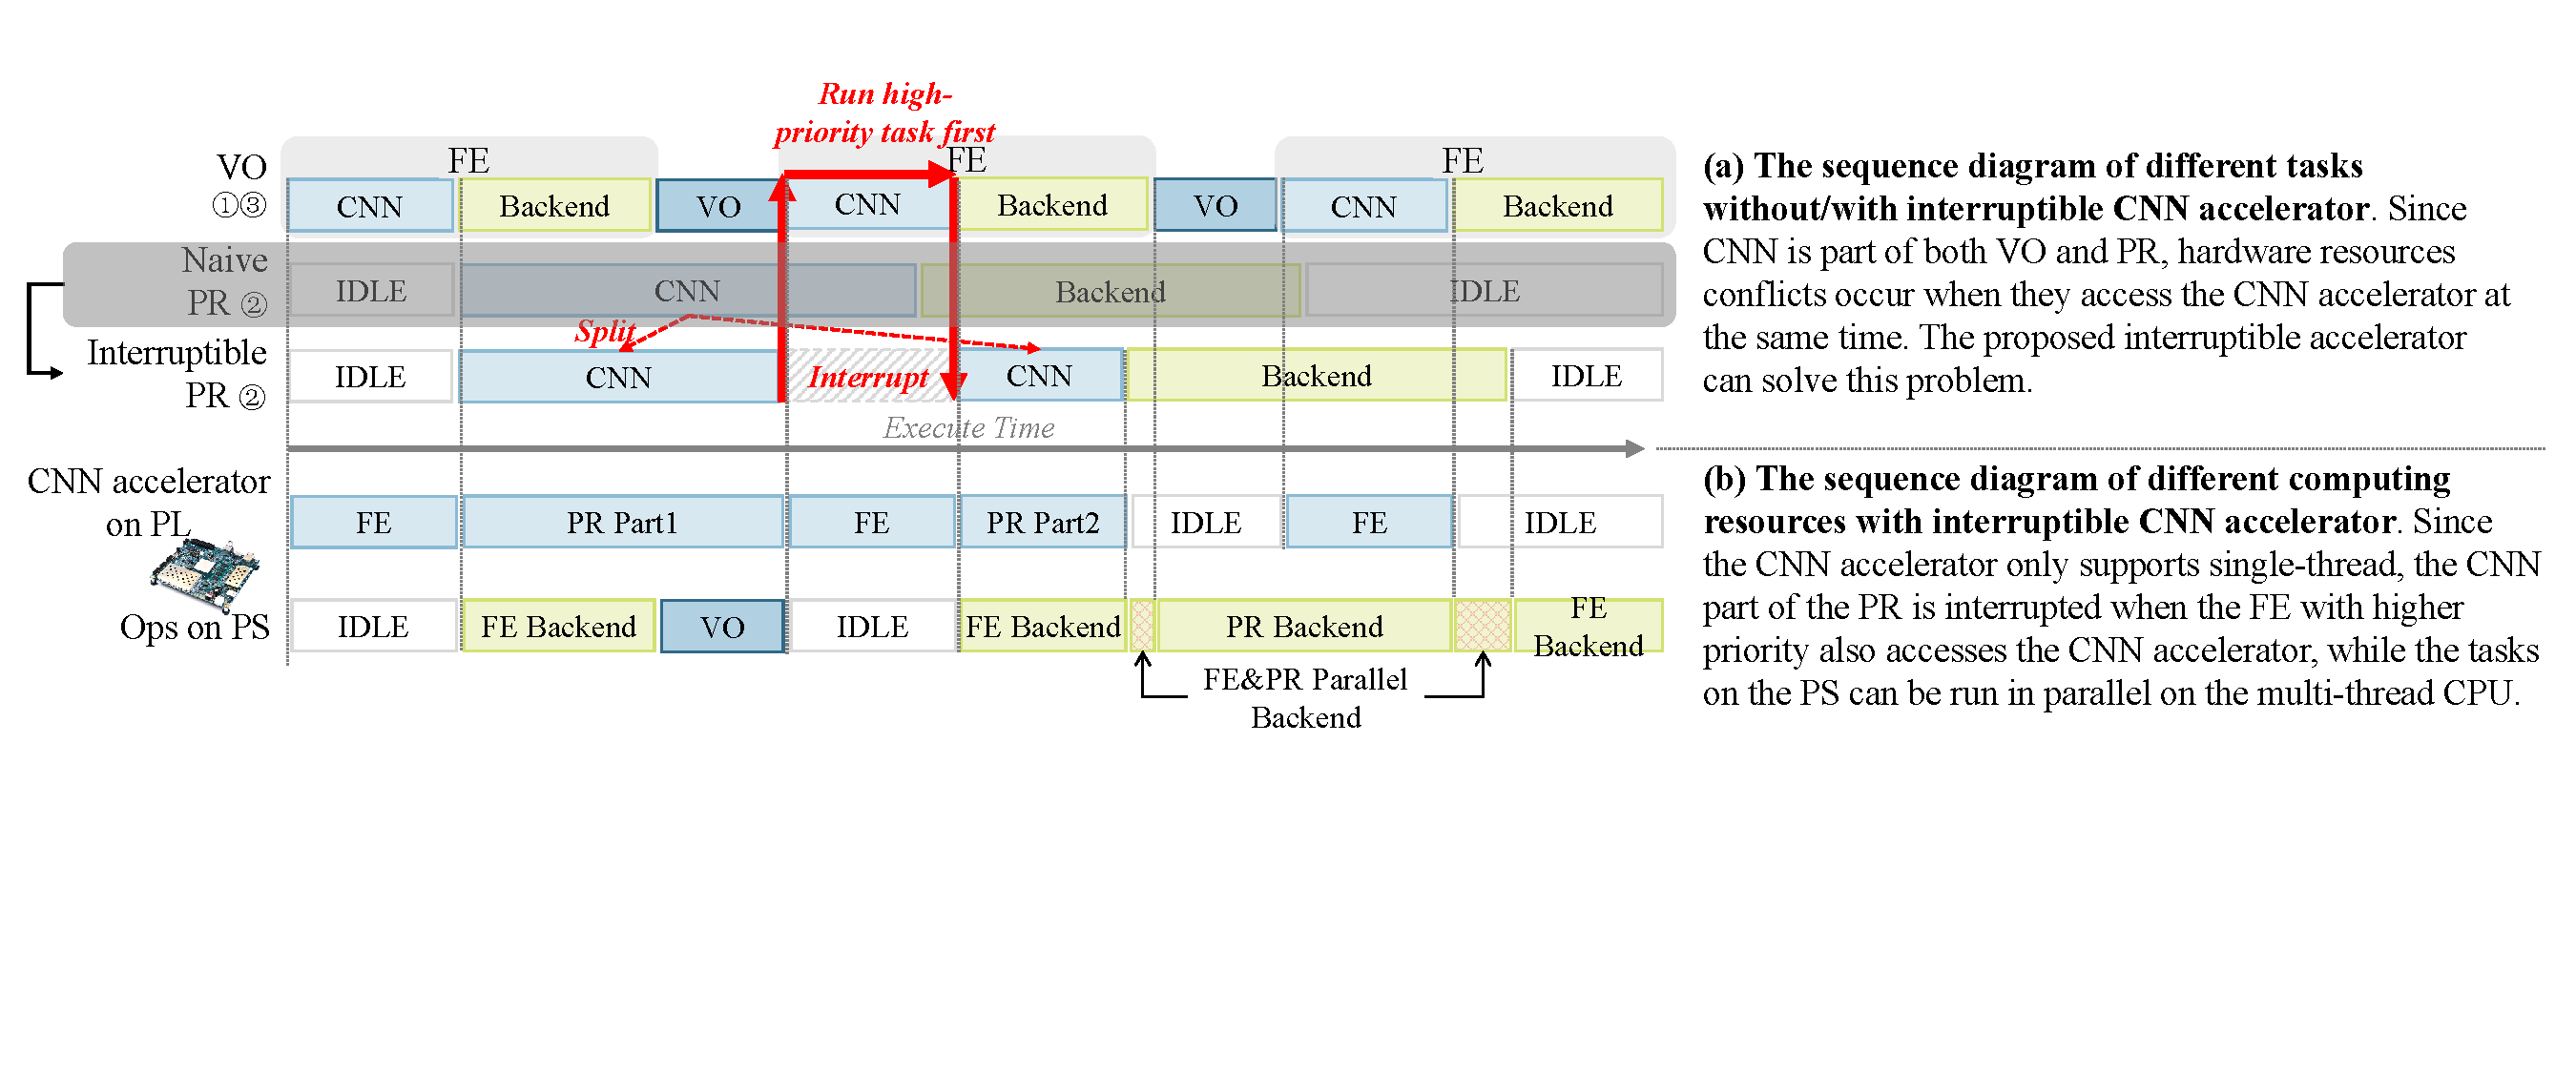
\includegraphics[width=0.99\linewidth]{fig/interDPR.eps}
% 	\caption{Interruption to solve the hardware resources conflicts.  When a high-priority task (FE) is started before the low-priority task (PR) is completed, the CNN accelerator backs up the status of PR to memory, and processes the FE task. When the high-priority task is completed, the low-priority task resumes and continues.
%     }
% 	\label{fig:interDPR}
% \end{figure*}


\begin{table*}[t]
	\caption{Description for the basic instructions.}
	\footnotesize
	\centering
% Table generated by Excel2LaTeX from sheet 'Sheet3'
%\linespread{1.1}\selectfont
\begin{tabular}{|p{2.7em}|m{3.7em}|m{14.2em}|m{4.2em}<{\centering}|m{4.2em}<{\centering}|m{4em}<{\centering}|m{4em}<{\centering}||m{6em}<{\centering}|m{6em}<{\centering}|}
	\hline
	\multicolumn{1}{|c|}{Category} & \multicolumn{1}{c|}{Type} & \multicolumn{1}{c|}{Description} & \multicolumn{1}{c|}{Address 1} & \multicolumn{1}{c|}{Address 2} & \multicolumn{1}{c|}{Address 3} & \multicolumn{1}{c||}{Workload} & \multicolumn{1}{c|}{Backup} & \multicolumn{1}{c|}{Recovery} \\
	\hline
	\multirow{2}[4]{*}{LOAD} & LOAD\_W & Load weights/bias from DDR to on chip weight buffer. & Off-chip Addr & Weights-buffer Addr & -     & Data  Length & -     & Weight / Inputdata \\
	\cline{2-9}\multicolumn{1}{|c|}{} & LOAD\_D & Load input data from DDR to on-chip data buffer. & Off-chip Addr & Data-buffer Addr & -     & Data  Length & -     & Weight / Inputdata \\
	\hline
	\multirow{2}[4]{*}{CALC} & CALC\_I & Calculate intermediate results (from partial input channels) for some output channels from partial  input channels. & Input  Data Addr & Intermediate Data Addr & Weight Addr & Calc Size & Previous final results / Intermediate data  & Weight / Inputdata /  Intermediate data \\
	\cline{2-9}\multicolumn{1}{|c|}{} & CALC\_F & Calculate the results for some output channels from all input channels. The pooling, bias-adding and element-wise operations are operated in this instructions. & Input  Data Addr & Output  Data Addr & Weight Addr & Calc Size & Final results & Inputdata \\
	\hline
	SAVE  & SAVE  & Save the results from on-chip data buffer to DDR. & Off-chip Addr & Data-buffer Addr & -     & Data  Length & -     & Inputdata \\
	\hline
	\end{tabular}%
	
	\label{tab:instr}%
  \end{table*}%


\begin{figure}[t]
	\centering
    % \vspace{-0.1cm} 
    % \setlength{\abovecaptionskip}{0cm} 
    % \setlength{\belowcaptionskip}{-0.6cm} 
	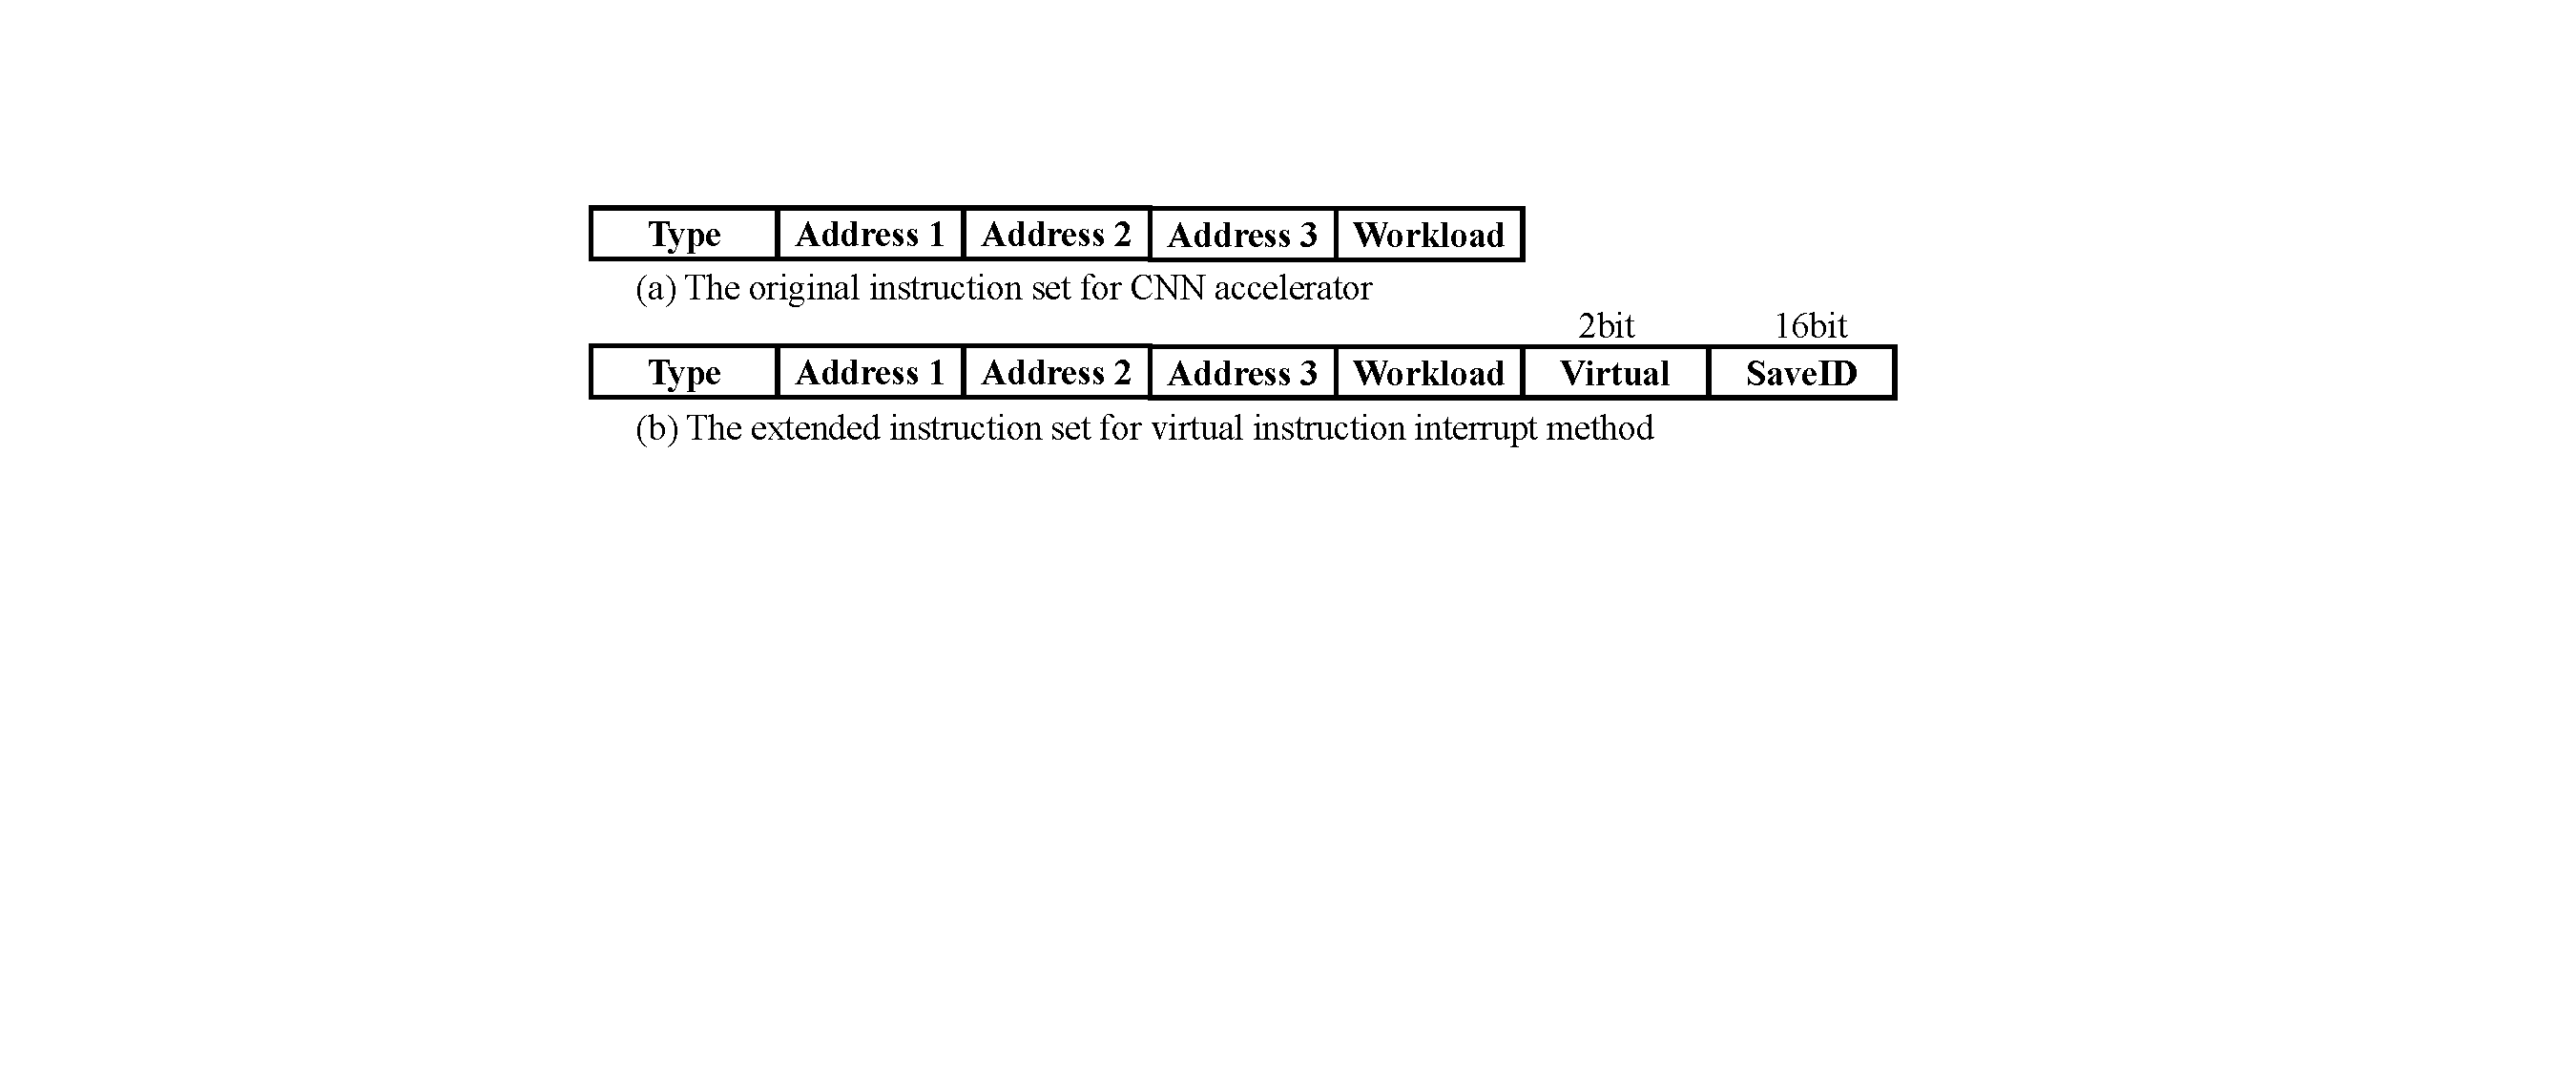
\includegraphics[width=0.99\linewidth]{fig/instructions.pdf}
	\vspace{-6mm}
	\caption{Fig(a), Original ISA. Fig(b), Virtual-Instruction ISA (VI-ISA).}
	\label{fig:instructions}
\end{figure}

In this section, we introduce our \textbf{virtual-instruction-based} method (VI method) to enable accelerator interrupt. 
\textcolor{blue}{
Compared with the CPU-Like and Layer-by-Layer interrupt method, virtual-instruction-based method enables interrupt inside each layer to avoid high interrupt response latency and only transfers the minimum amount of data for backup and restore to lower the extra cost of the interrupt.
}


% In this section, we introduce our virtual-instruction-based method to enable accelerator interrupt. To minimize the interrupt response latency and extra cost for interrupt, we propose the virtual-instruction-based accelerator interrupt method.

\subsection{ Instruction Driven Accelerator }
\label{sec:instrAcc}
There are three categories of instruction in the instruction-driven accelerator: LOAD, CALC, and SAVE  ~\cite{guo2017angel,qiu2016going,yu2018instruction}. The instruction description of each kind of instruction is listed in \Cref{fig:instructions}(a) and \Cref{tab:instr}.

The LOAD instruction moves input featuremaps and weights from DDR to on-chip memory. The SAVE instruction moves the calculated output features from on-chip memory to DDR. 

Each CALC  instruction,  including CALC\_I and CALC\_F, processes the convolution according to the hardware parallelism with $Para_{height}$ lines from $ Para_{in} $ input channels to $ Para_{out}$ output channels. $Para_{height}$, $ Para_{in} $, and $ Para_{out} $ are the parallelism along the height, input channel and output channel dimensions, which is determined by the hardware and original ISA.

\Cref{fig:singlesave}(a) illustrates the operation of CALC instructions. The convolution of the last $ Para_{in} $ input channels is CALC\_F, and the convolutions for the former input channels are CALC\_I. The CALC\_F and the CALC\_I instructions for the same output channels, as well as the LOAD instructions for corresponding input featuremaps and weights, are considered as a \textbf{CalcBlob}  (\Cref{sec:exampleVirtual}(c) lists an example for CalcBlob). In each CalcBlob, there is a LOAD\_W instruction for the corresponding weights. 
\textcolor{blue}{
However, when there are only few input channels (such $Ch_{in} = Para_{in}$), all input data required by a CalcBlob can be fetched to the chip by a single LOAD\_D. 
During the CalbBlob execution, the input buffer remains unchanged. 
For the next CalcBlob, since the required input data is exactly the same, there is no need to execute a LOAD\_D.
Thus, some CalcBlobs do not have  LOAD\_D instruction.
}


% Each CALC  instruction,  including CALC\_I and CALC\_F processes the convolution according to the hardware parallelism.
% Each CALC instruction, including CALC\_I and CALC\_F processes the convolution from input feature of the hardware input parallelism ($Para_{in}$) to the output feature of the hardware output parallelism ($ Para_{out}$), as illustrated in \Cref{fig:singlesave}(a). The convolution of the last input channels is CALC\_F, and the convolutions for the former input channels are CALC\_I. The CALC\_F and the CALC\_I instructions to generate the output channels, as well as the LOAD instructions for corresponding input featuremaps and weights are considered as a \textbf{CalcBlob}. Besides the convolution, some other operations like pooling is also represented in the CALC\_F instruction.

% Considerring to the limited on-chip data memory, the on-chip data buffer may not able to store all of the input and output featuremaps. To solve this problem, a CALC instruction is not designed for the entile featuremap, yet servel lines of the featuremap. The parallelism along the height dimension of a CALC instruction is denoted as  





% \subsection{Accelerator Interrupt }

\subsection{How To Interrupt: Virtual Instruction}
\label{sec:howinter}

As illustrated in \Cref{fig:singlesave}(e),there are four stages to handle interrupt, including: (1) Time for finishing the current operation, $t1$. (2) Time to backup, $t2$. (3) Time for the high-priority task, $t3$. (4) Time to restore the low-priority task ,$t4$. 
The latency to respond the interrupt is $t_{latency} = t_1+t_2$. The extra cost for interrupt is $t_{cost}=t_2+t_4$. For the instruction flow illustrated in \Cref{fig:singlesave}(c), the interrupt stages are shown in \Cref{fig:singlesave}(e).
There are different methods to implement interrupt in CNN accelerators.

\textbf{CPU-Like.}
When an interrupt request occurs in CPU, CPU backs up all the on-chip registers to DDR. However, there are only tens of registers in CPU, and the volume of the backed-up data is less than 1 KB  ~\cite{furber2000arm}. In CNN accelerators, there are hundreds of KB $\sim$ several MB on-chip caches  ~\cite{qiu2016going, guo2017angel} to store input featuremaps or weights. 
% If all on-chip caches are backed-up/recovered, the cost of data transfer in the accelerator is much higher than that of CPU. 
Thus, the extra data transfer increases both the interrupt response latency ($t_{latency}$) and the additional cost ($t_{cost}$).

\textbf{Layer-by-layer.}
Most accelerators run the CNN layer by layer  ~\cite{qiu2016going,guo2017angel}. 
There is no extra data transfer for the accelerator to switch between different tasks after each layer, thus, $t_{cost}=0$. 
However, the position of the interrupt request is irregular and unpredictable. When an interrupt occurs inside a CNN layer, the CNN accelerator needs to finish the whole layer before switching, which leads to the high response latency ($t_{latency}$).

% The latency to respond the interrupt and the performance degradation of the CPU-like interrupt and Layer-by-layer method will be evaluated in \Cref{sec:experiments}.



We propose the \textbf{virtual-instruction-based} method (VI method) to enable low-latency interrupt. 
% Different from the CPU-like interrupt, which backup/recovery all the on-chip caches, only the on-chip cache which is still needed in future execution will be backed-up and restored. So that the amount of data transfer is much lower than that of CPU-like interrupt.
To reduce the interrupt response latency, our virtual-instruction-based method is interruptible inside each layer. We add some virtual instructions to the original instruction sequence to enable the interrupt.
The virtual instructions, which contain the backup and recovery instructions, are responsible for backing up and restoring on-chip caches. 

\textbf{Virtual SAVE} instructions back up the intermediate results from partial input channels or the final output results. There is no need to back up the input featuremaps and weights, because these inputs are already stored in DDR. 

\textbf{Virtual LOAD} instructions restore the input featuremaps from DDR to on-chip caches.
% because input featuremaps are loaded by one CalcBlob, and shared across subsequent CalcBlobs, and thus the subsequent CalcBlobs do not read the input featuremaps. 
Virtual LOAD instructions also need to restore the intermediate results from partial input channels backed up by the virtual SAVE instructions.

% By adding the virtual instructions, the CNN can be interrupted anywhere, and the latency to respond interrupt is reduced.


% For backup virtual instructions, the corresponding input data and weights are already stored in DDR. 
% Thus, there is no need to back up the input buffer and weight buffer. Only the intermediate data and the final output results are needed to be backed-up. 

% For recovery virtual instructions, the weights and input data, as well as the backed-up intermediate data, are needed to be restored from DDR to the on-chip cache.
% The accelerator can switch to a different task after the backup virtual instructions, and resume the execution by the recovery virtual instructions.

% By adding the virtual instructions, the CNN can be interrupted anywhere, and the latency to to response the interrupt is reduced. However, there virtual instructions are only valid when interrupt occurs. So we add a field in the origin instruction set, that indicates whether the instruction a virtual instruction. If no interrupt occurs, virtual instructions will be skipped and discarded, which can ensure the efficiency of uninterrupted execution. The modifications to the instruction set will be introduced in \Cref{sec:virtualinstr}. 


% However, the CPU-like interrupt would back up all the on-chip registers to DDR. In CPU, there are tens of registers, and the backed-up data is around 1 KB. In CNN accelerators, there are hundreds of KB ~ several MB on-chip cache  ~\cite{qiu2016going, yu2018instruction}. If all the on-chip cache is backed-up and recovered, the cost of data transfer in the CNN accelerator is much higher than that of CPU.

% We propose the \textbf{virtual-instruction-based} method to enable low-latency interrupt. The low-priority task maintains the executing status itself, rather than the hardware or the interrupt handler used in CPU. Only the cache which is still needed in future execution will be backed-up and restored.

% The virtual instructions, which contain the backup and recovery instructions, are generated in the compilation phase, together with the normal instructions. 
% For backup instructions, the corresponding input data and weights are still stored in DDR. 
% There is no need to back up the input buffer and weight buffer, and only the intermediate data and the final output results are needed to be backed-up. 
% For recovery instructions, the weights and input data for future calculation, as well as the backed-up intermediate data, are needed to be restored from DDR to the on-chip cache.

% There is a field in the instruction set, that indicates whether the instruction a virtual instruction. If no interrupt occurs, virtual instructions will be skipped and discarded, which can ensure the efficiency of uninterrupted execution.







\begin{figure*}[t]
    % \flushleft
    \centering
    % \vspace{-0.1cm} 
    % \setlength{\abovecaptionskip}{0cm} 
    % \setlength{\belowcaptionskip}{-0.05cm} 
	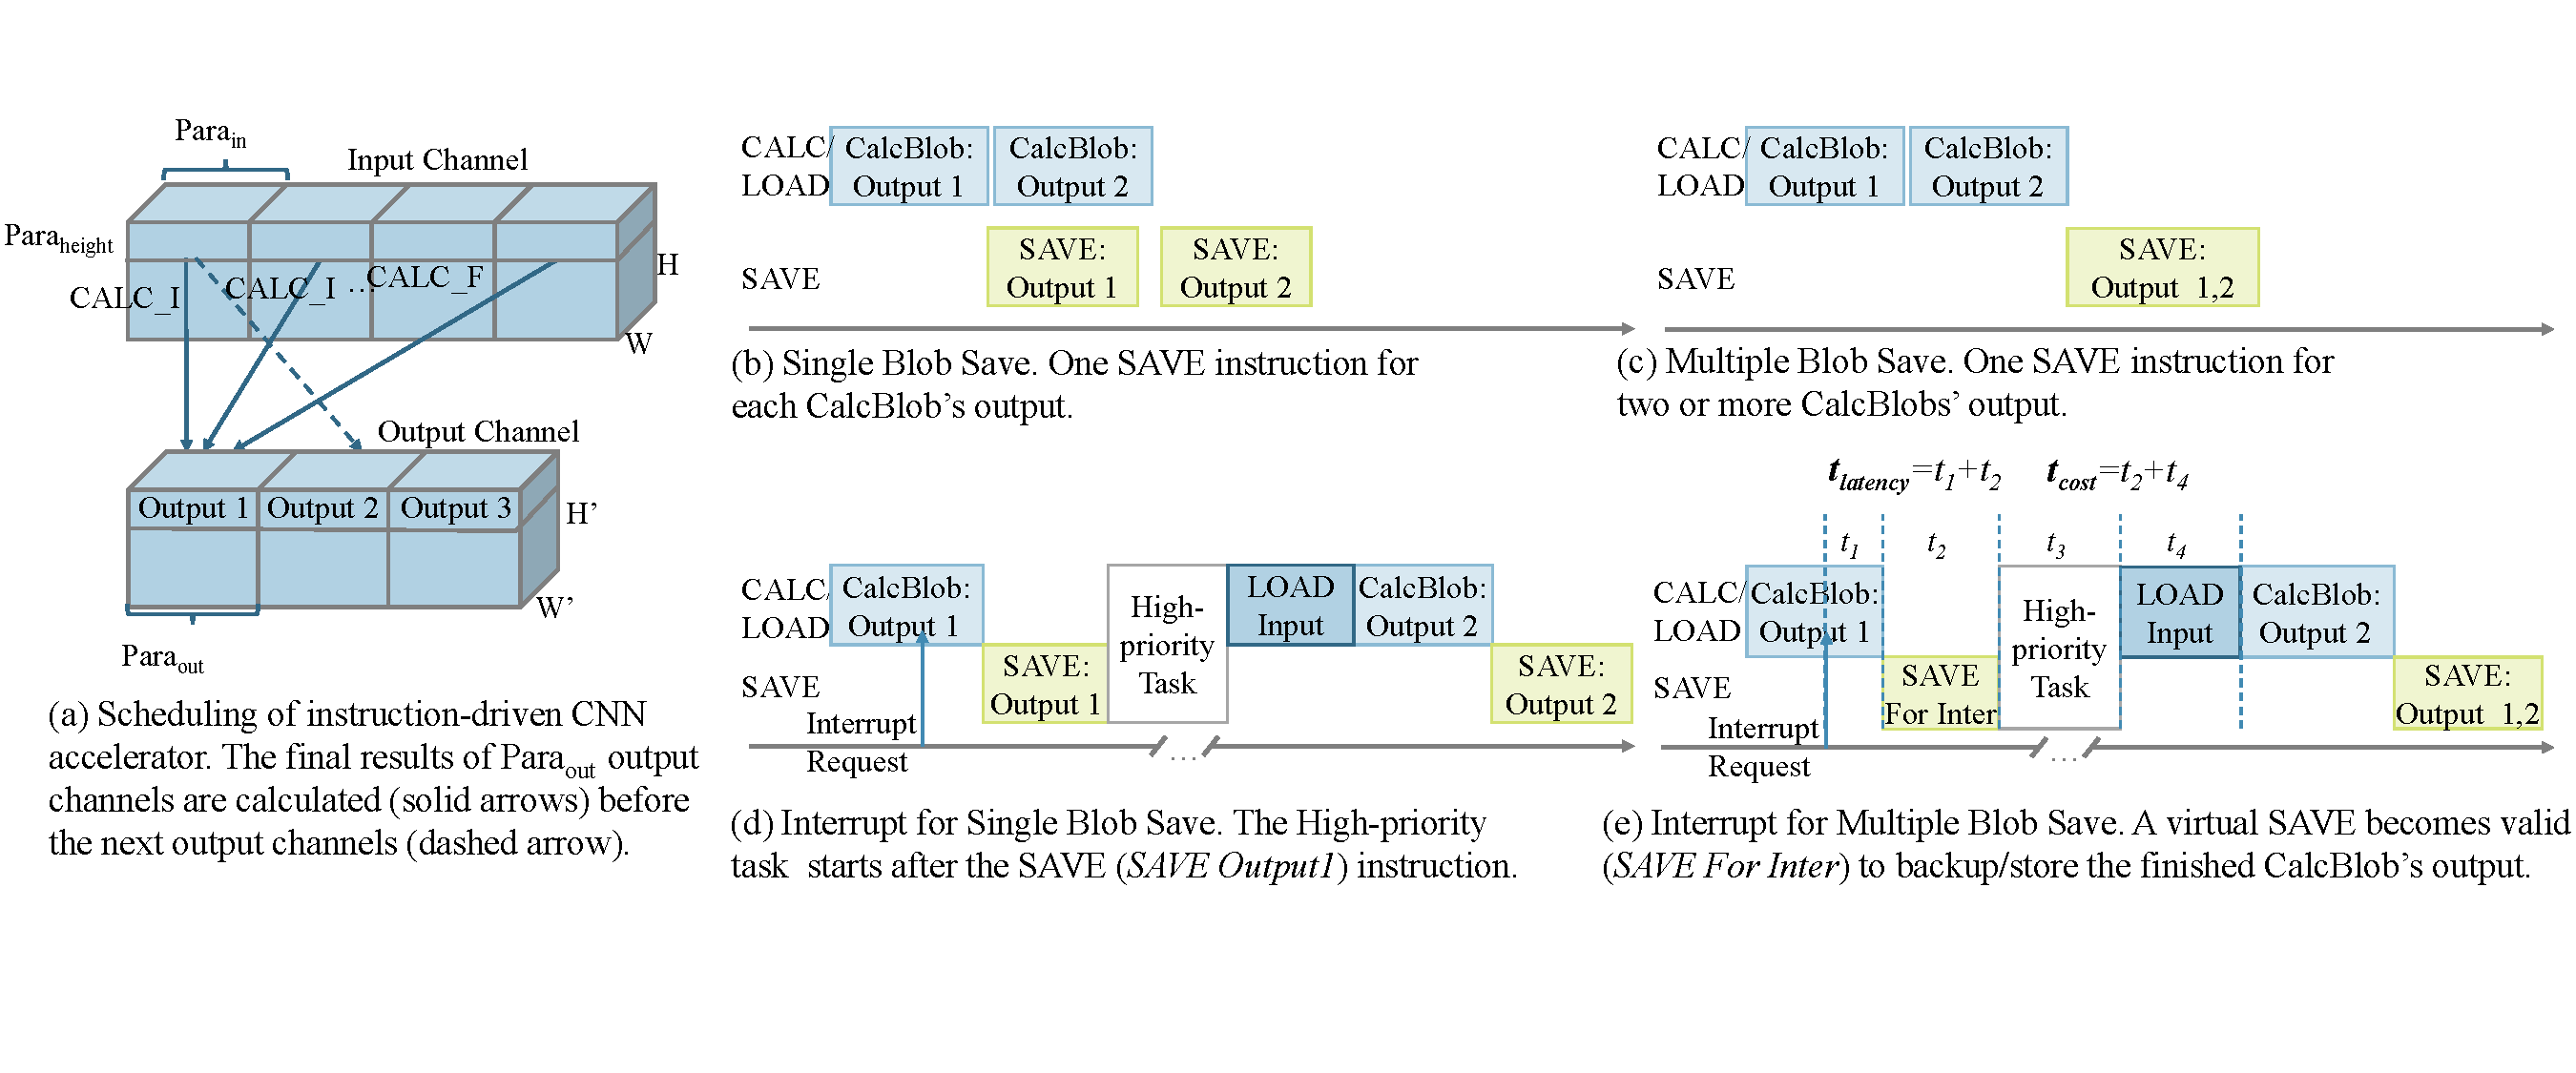
\includegraphics[width=0.99\textwidth]{fig/singlesave.pdf} 	
	\vspace{-1mm} 
    \caption{
		Illustration of scheduling on the CNN accelerator. Fig(a), a CalcBlob is the instructions that calculate the final results of $Para_{out}$ output channels from all input channels (the set of solid arrows). Fig(b), one SAVE instruction is only responsible for saving the results of one CalcBlob. Fig(c), one SAVE instruction is responsible for saving the results of several CalcBlobs. Fig(d) and Fig(e) illustrate the accelerator interrupt of Fig(b) and Fig(c). The latency ($t_{latency}$) and extra cost ($t_{cost}$) are labelled in Fig(e).
    }
	\label{fig:singlesave}
\end{figure*}



\subsection{ Where To Interrupt: After SAVE/CALC\_F }
\label{sec:whereinter}
The virtual-instruction-based method has two potential factors that may lead to system performance degradation: 1) The extra data transfer to backup/restore running status takes up additional bandwidth resources. 2) The instruction fetching for the virtual instructions also uses bandwidth resources.
%  Even they are skipped and discarded.
To address the above problems of virtual-instruction-based method, we analyze the interrupt cost and select the positions of adding the virtual instructions.
The backup/recovery data for different interrupt positions at each kind of instruction are listed in the Backup/Recovery columns of \Cref{tab:instr}. The backup/recovery data transfer for each instruction is analyzed as follows:

\textbf{LOAD\_W / LOAD\_D. }
When an interruption occurs at LOAD, the newly loaded data are immediately flushed when running the high-level CNN, leading to bandwidth waste.

\textbf{CALC\_I.} 
When an interrupt occurs at CALC\_I, the unsaved final results (generated by previous CALC\_F) should be saved to DDR. The intermediate data from current CALC\_I should also be sent to DDR for further use. At the Recovery stage, the intermediate data should be fetched from DDR. The data movement of intermediate results leads to additional bandwidth requirements.


\textbf{CALC\_F.}
When an interrupt occurs at CALC\_F, there are no intermediate results. 
Although it is necessary to back up the unsaved final results which are generated by previous CALC\_F, these results will be stored in DDR through the subsequent original SAVE instruction.
If the accelerator can record the interrupt status, we can modify the address and workload when executing subsequent original not-virtual save instruction.
In this way, we can avoid the repetitive transmission of the final output results.
% The state records and modifications to normal SAVE instruction will be introduced in the following subsections.
The input data are shared across the CalcBlobs. Thus, the recovery virtual instruction needs to restore the shared input featuremaps.



\textbf{SAVE.}
The overhead of interrupt is only to transfer input data from DDR to the on-chip caches. 

In order to minimize the cost of interrupt, we make the CNN interruptible after the SAVE or CALC\_F. This method only introduces extra data transfer to recovery input data without any extra backup data ($t_2 = 0$). Thus, $t_{cost} = t_4$, in our virtual-instruction-based interrupt.

% Additional virtual instructions also take up bandwidth at instruction fetching phase, even if they are not executed. The instruction number of CALC\_I is tens of times of that of SAVE/CALC\_F. If the network can be interrupted after each CALC\_I, the rapidly increasing virtual instructions reduce the system performance.


\begin{figure*}[t]
	\centering
	\subfloat[$t_1$ for Layer-by-Layer method.]{
		\begin{minipage}[t]{0.45\linewidth}
			\centering
	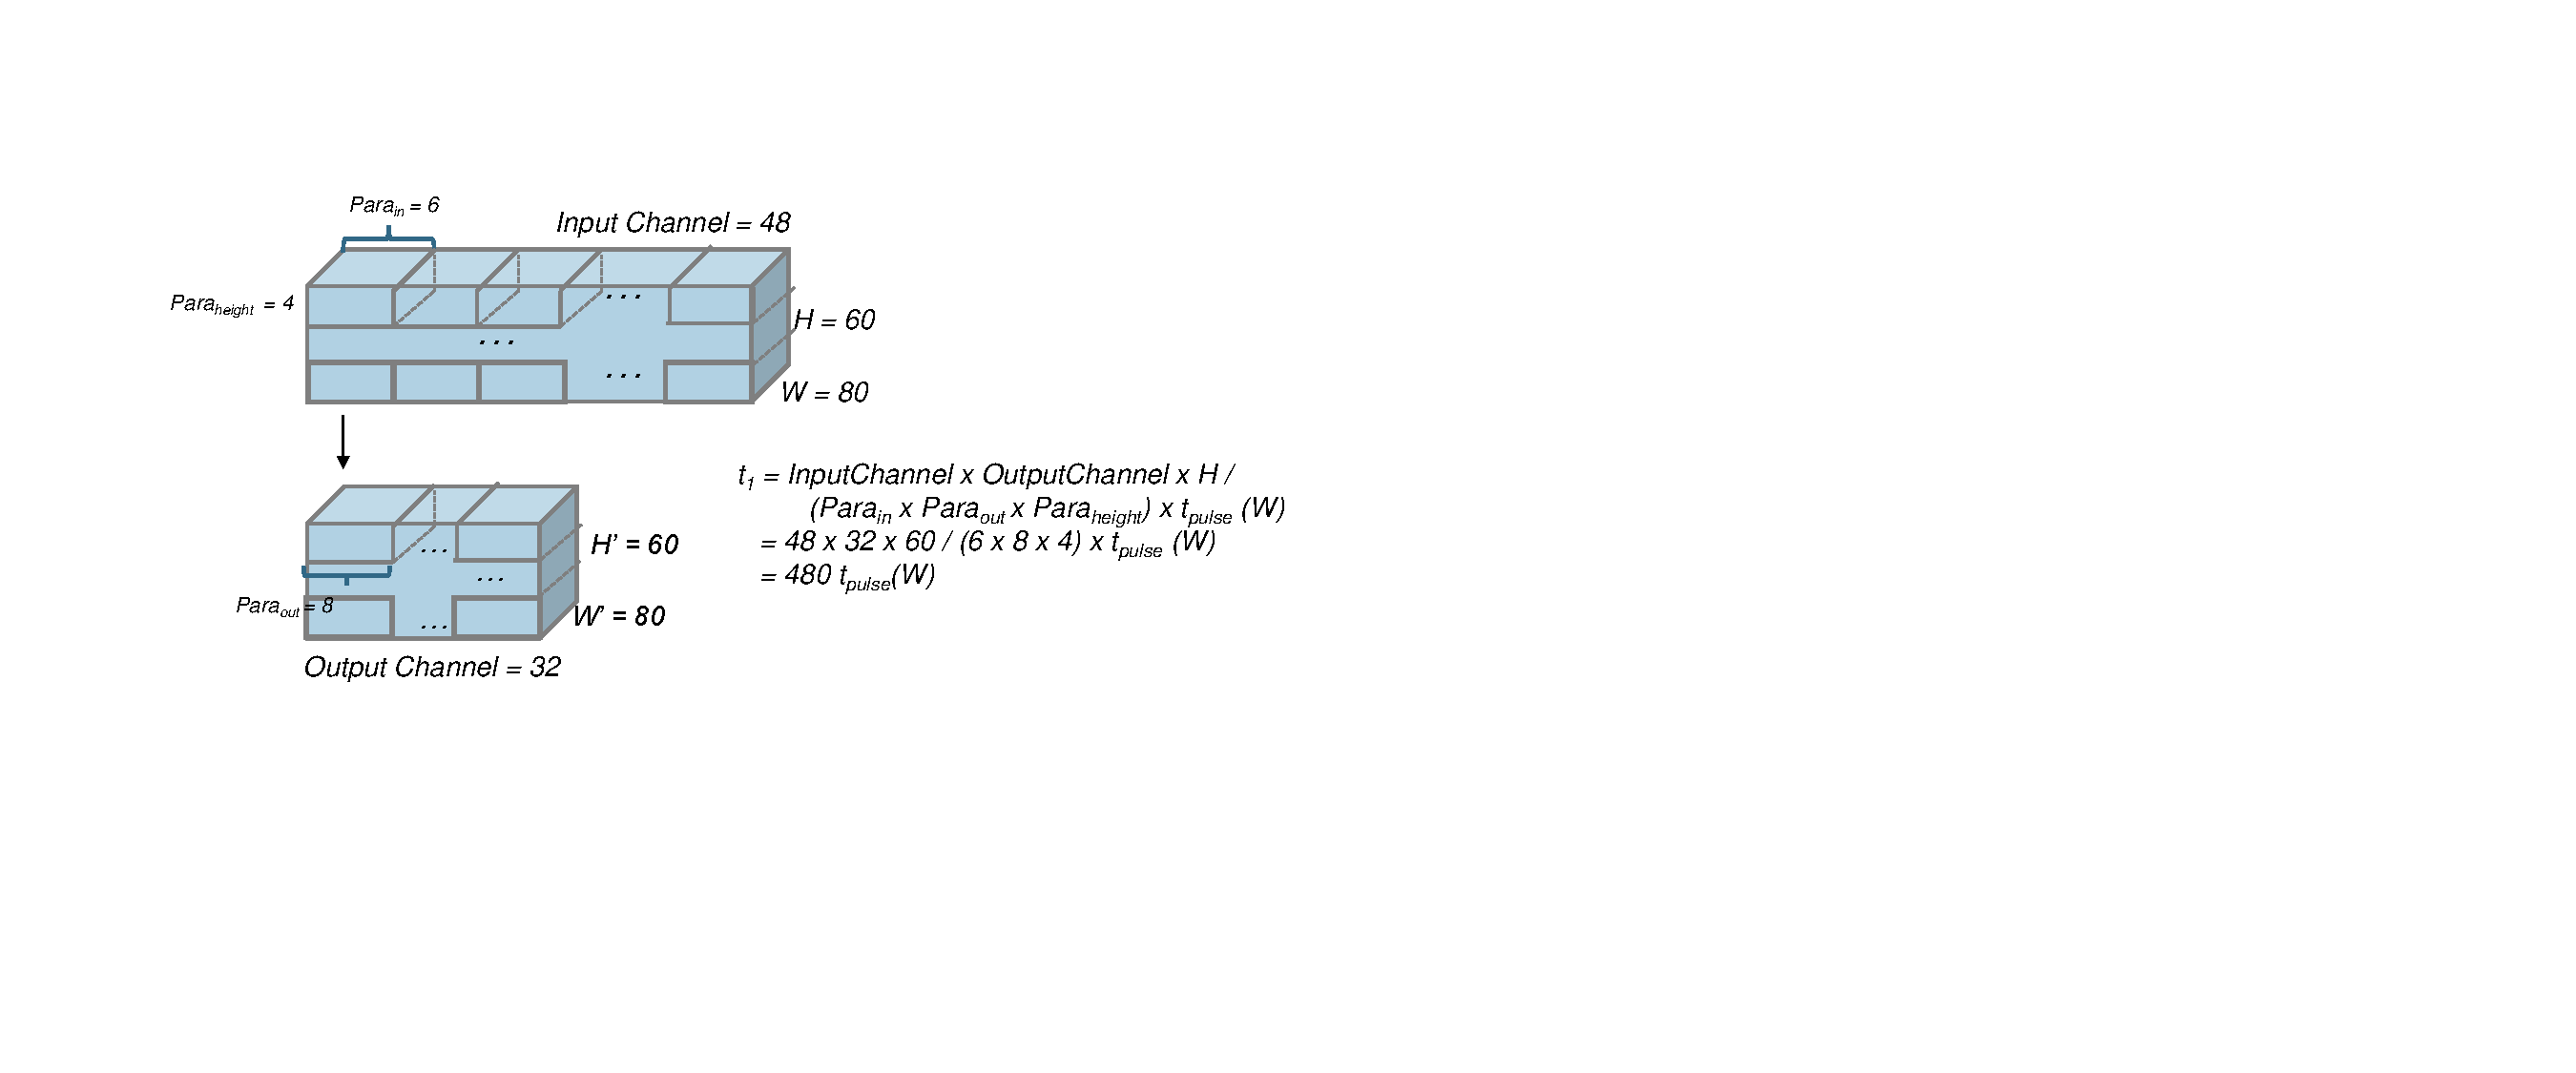
\includegraphics[width=0.99\linewidth]{fig/t1all.pdf}
		\end{minipage}%
	}
	\subfloat[$t_1$ for Virtual-Instruction method]{
		\begin{minipage}[t]{0.45\linewidth}
			\centering
	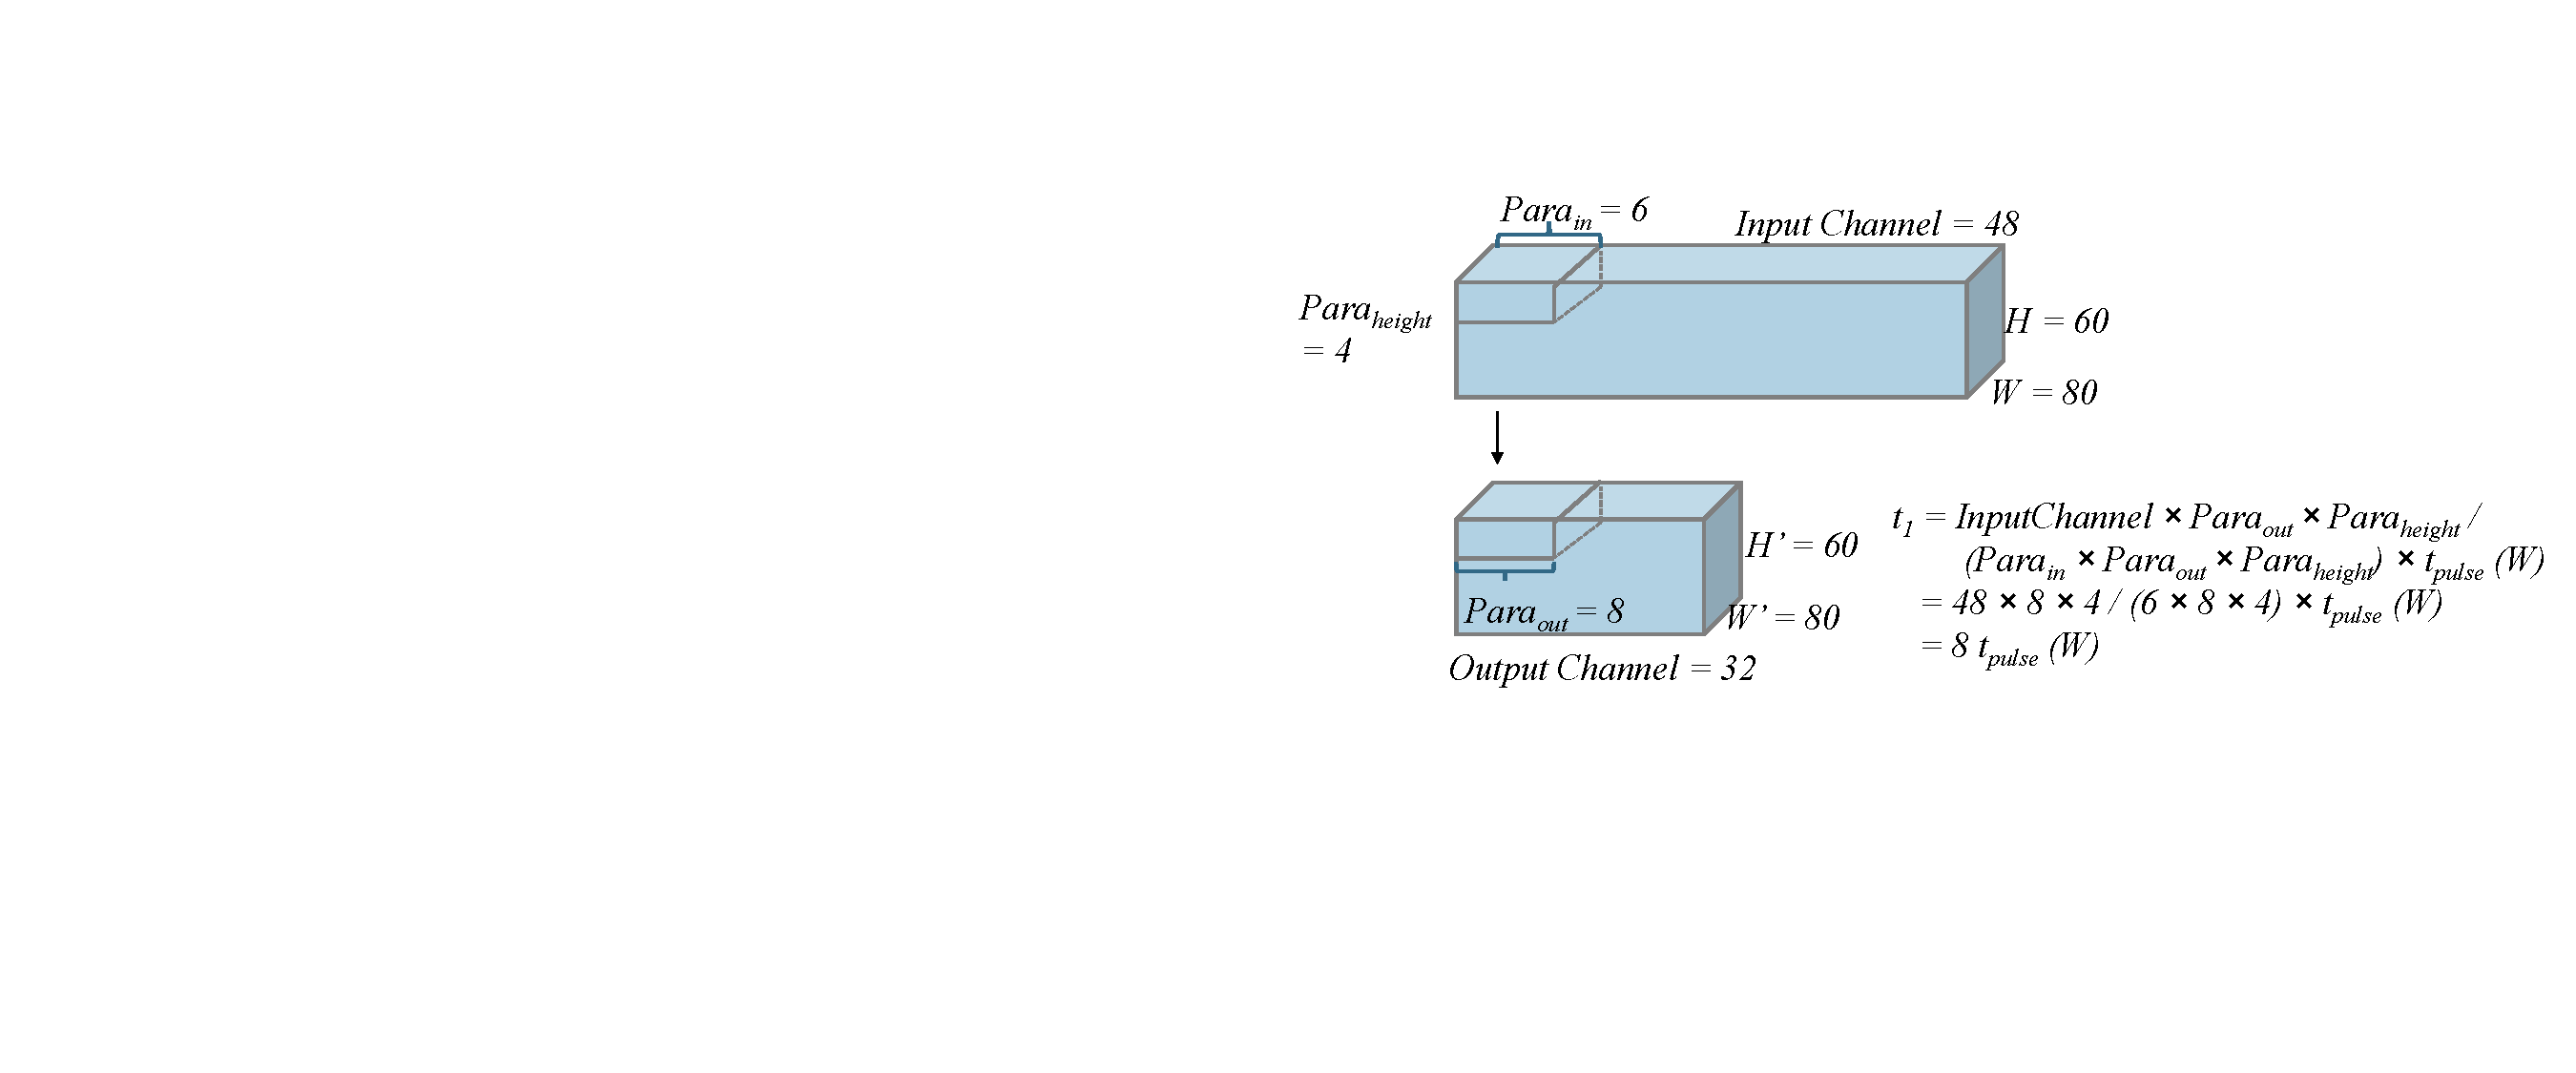
\includegraphics[width=0.99\linewidth]{fig/t1after.pdf}
		\end{minipage}%
	}
	\vspace{-1mm} 
	\caption{ An example of waiting time for finishing the current operation ($t_1$) in a convolution layer. Compared with the Layer-by-Layer method, the waiting time of our Virtual-Instruction method is reduced to $1.6\%$ in this example. The reduction in latency is related to the height ($H$) of the input featuremaps.  }
	\label{fig:t1example}
\end{figure*}



\subsection {Latency Analysis}

In this subsection, we quantitatively analyze the impact of interruptible position on interrupt respond latency. 
As introduced in \Cref{sec:instrAcc}, each CALC  instruction processes the convolution according to the hardware parallelism with $Para_{height}$ lines from $ Para_{in} $ input channels to $ Para_{out}$ output channels. 
We here note the computation of a CALC instruction an $instruction pulse$, or $pulse$.
The computation time of each pulse is related to the hardware architecture and the width of the convolution layer. The larger the width, the larger the workload of a single calculation instruction, and thus the CALC instruction consumes more time. We note the time consumption of a pulse as a function of the featuremap width, $t_{pulse}$:

\begin{equation}
	t_{pulse}(W) = t_{hw} \times W
\end{equation}

$t_{hw}$ indicates the time for hardware to produce the intermediate results of one pixel, which is defined by the hardware design and the clock frequency. $W$ is the width of the featuremaps, indicating the workload of the instruction.

\Cref{fig:t1example}(a) shows the worst case of waiting for finishing the current operation of the Layer-by-Layer interrupt method. The worst case is that the interrupt request occurs at the beginning of the layer. In this case, the accelerator will wait until finishing the whole layer. The calculation of the whole layer consists of $N_{pulse\_layer}$ successive CALC instructions. We note the worst time of waiting to finish the current layer, which is the total time of these pulses, as $t_{1\_layer}$.

\begin{equation}
	\small
	N_{pulse\_layer} = \frac{ Ch_{in} \times Ch_{out} \times H }{ (Para_{in} \times Para_{out} \times Para_{height}) } 
\end{equation}

\begin{equation}
t_{1\_layer} = N_{pulse} \times t_{pulse}(W)
\end{equation}

$Ch_{in}$ and $Ch_{out}$ is the number of input channels and output channels. $H$ is the height of featuremaps.

On the other hand, if the execution of the CNN accelerator can be interrupted after SAVE/CALC\_F instructions, the worst case of waiting for finishing the current operation is illustrated in \Cref{fig:t1example}(b). The calculation of the whole CalcBlob consists of $N_{pulse\_VI}$ successive CALC instructions. We note the worst waiting time in this case as $t_{1\_VI}$.

\begin{equation}
	\small
	N_{pulse\_VI} = \frac{ Ch_{in} \times Para_{out} \times Para_{height} }{ (Para_{in} \times Para_{out} \times Para_{height}) } 
\end{equation}

\begin{equation}
t_{1\_VI} = N_{pulse\_VI} \times t_{pulse}(W)
\end{equation}


Because our Virtual-Instruction method (VI method) only interrupts the execution after CALC\_F and SAVE, there is no extra data transfer for the intermediate results. The backup operation in the VI method only transfers the final results, which are also transfered to DDR with the SAVE instructions in the Layer-by-Layer method. 
Experimental results, which will be given in \Cref{sec:expt1t2}, show that the data transfer time for the final results is much less than the calculation time (less than 20\%), in both the Layer-by-Layer method and the VI method. Thus the latency to respond to the interrupt request ($t_{latency}$) is mainly determined by the time of finishing the current operation.

As the interrupt request is unpredictable, we model the interrupt location as evenly distributed within each layer. Thus the average interrupt latency is $\bar{t}_{latency} $.

\begin{equation}
	\bar{t}_{latency}  \simeq \frac{1}{2} \times t_{1}
\end{equation}

Compared with the Layer-by-Layer method, the latency of our method is reduced to $R_l$.

\begin{equation}
	\small
	\begin{split}
	R_l & =  \frac{\bar{t}_{latency\_VI}}{\bar{t}_{latency\_layer}} \simeq \frac{\frac{1}{2} \times t_{1\_VI}}{\frac{1}{2} \times t_{1\_layer}}  = \frac{ N_{pulse\_VI} \times t_{pulse}(W) }{ N_{pulse} \times t_{pulse}(W) }  \\
		   & = \frac{ N_{pulse\_VI} }{N_{pulse} } = \frac{ Ch_{in} \times Para_{out} \times Para_{height}  }{  Ch_{in} \times Ch_{out} \times H } \\
		   & = \frac{ Para_{out} \times Para_{height} }{ Ch_{out} \times H} 
	\end{split}
\end{equation}

$\bar{t}_{latency\_VI}$ and $\bar{t}_{latency\_VI}$ are the average interrupt latency of the Virtual-Instruction method and the Layer-by-Layer method. The effect of latency reduction of the VI method is related to the number of output channels ($Ch_{out}$) and featuremap height ($H$). The larger the featuremaps output channels and the height, the better latency reduction result can be achieved.

An example of a convolution layer with a typical size in CNN is given in \Cref{fig:t1example}. The parameters are labelled in the figures. The latency can be reduced to $R_t = 8/480 =1.6\%$.



\subsection{Virtual Instruction ISA (VI-ISA) }
\label{sec:virtualinstr}

We add two fields to the instruction set: 1) Virtual and 2) SaveID, as illustrated in \Cref{fig:instructions}(b). 

\textbf{   Virtual Field}. The virtual instructions should be only valid when interrupt occurs. So we add a field in the original ISA, that indicates whether the instruction is a virtual instruction. If no interrupt occurs, virtual instructions will be skipped and discarded, which can ensure the efficiency of uninterrupted execution. Three values can be set to Virtual Field:
% \begin{itemize}

	\textit{2'b00} indicates this instruction is not virtual, should always be executed.
	
	\textit{2'b01} indicates this instruction is the SAVE instruction for backup. When an interrupt occurs, the high-priority network will start after this instruction.
	
	\textit{2'b10} indicates this instruction is the LOAD instruction for recovery. The corresponding instructions will be executed after the high-priority network.
% \end{itemize}

\textbf{ SaveID Field }
SaveID links CalcBlob instructions to the corresponding SAVE. SaveID of each not-virtual SAVE instruction differs. If the generated outputs of CalcBlobs are stored to DDR by a SAVE instruction, the CalcBlobs have the same SaveID as the SAVE instruction.

% The SaveID for a CalcBlob is the same as its CALC\_F instruction.
One SAVE instruction can correspond to one CalcBlob (Single Blob Save, illustrated in \Cref{fig:singlesave}(b)) or multiple CalcBlobs (Multiple Blob Save, illustrated in \Cref{fig:singlesave}(c)).

For Single Blob Save, no virtual SAVE is added. The high-priority network can be started after the original not-virtual SAVE. The virtual LOAD instructions for data recovery are generated after the original SAVE, and executed after the high-priority network. The execution timeline is shown in \Cref{fig:singlesave}(d).

For Multiple Blob Save, virtual SAVE and LOAD instructions are generated after the CALC\_F of each CalcBlob. When the interrupt request occurs, the virtual SAVE instruction will be executed before the start of the high-priority network. Virtual LOAD instructions for data recovery are executed after the high-priority network. The subsequent original not-virtual SAVE instruction with the same SaveID as the CalcBlob will be modified to avoid duplicate output data transfer. The execution timeline is shown in \Cref{fig:singlesave}(e).


\begin{figure}[t]
	\centering
    % \vspace{-0.1cm} 
    % \setlength{\abovecaptionskip}{0cm} 
    % \setlength{\belowcaptionskip}{-0.4cm} 
	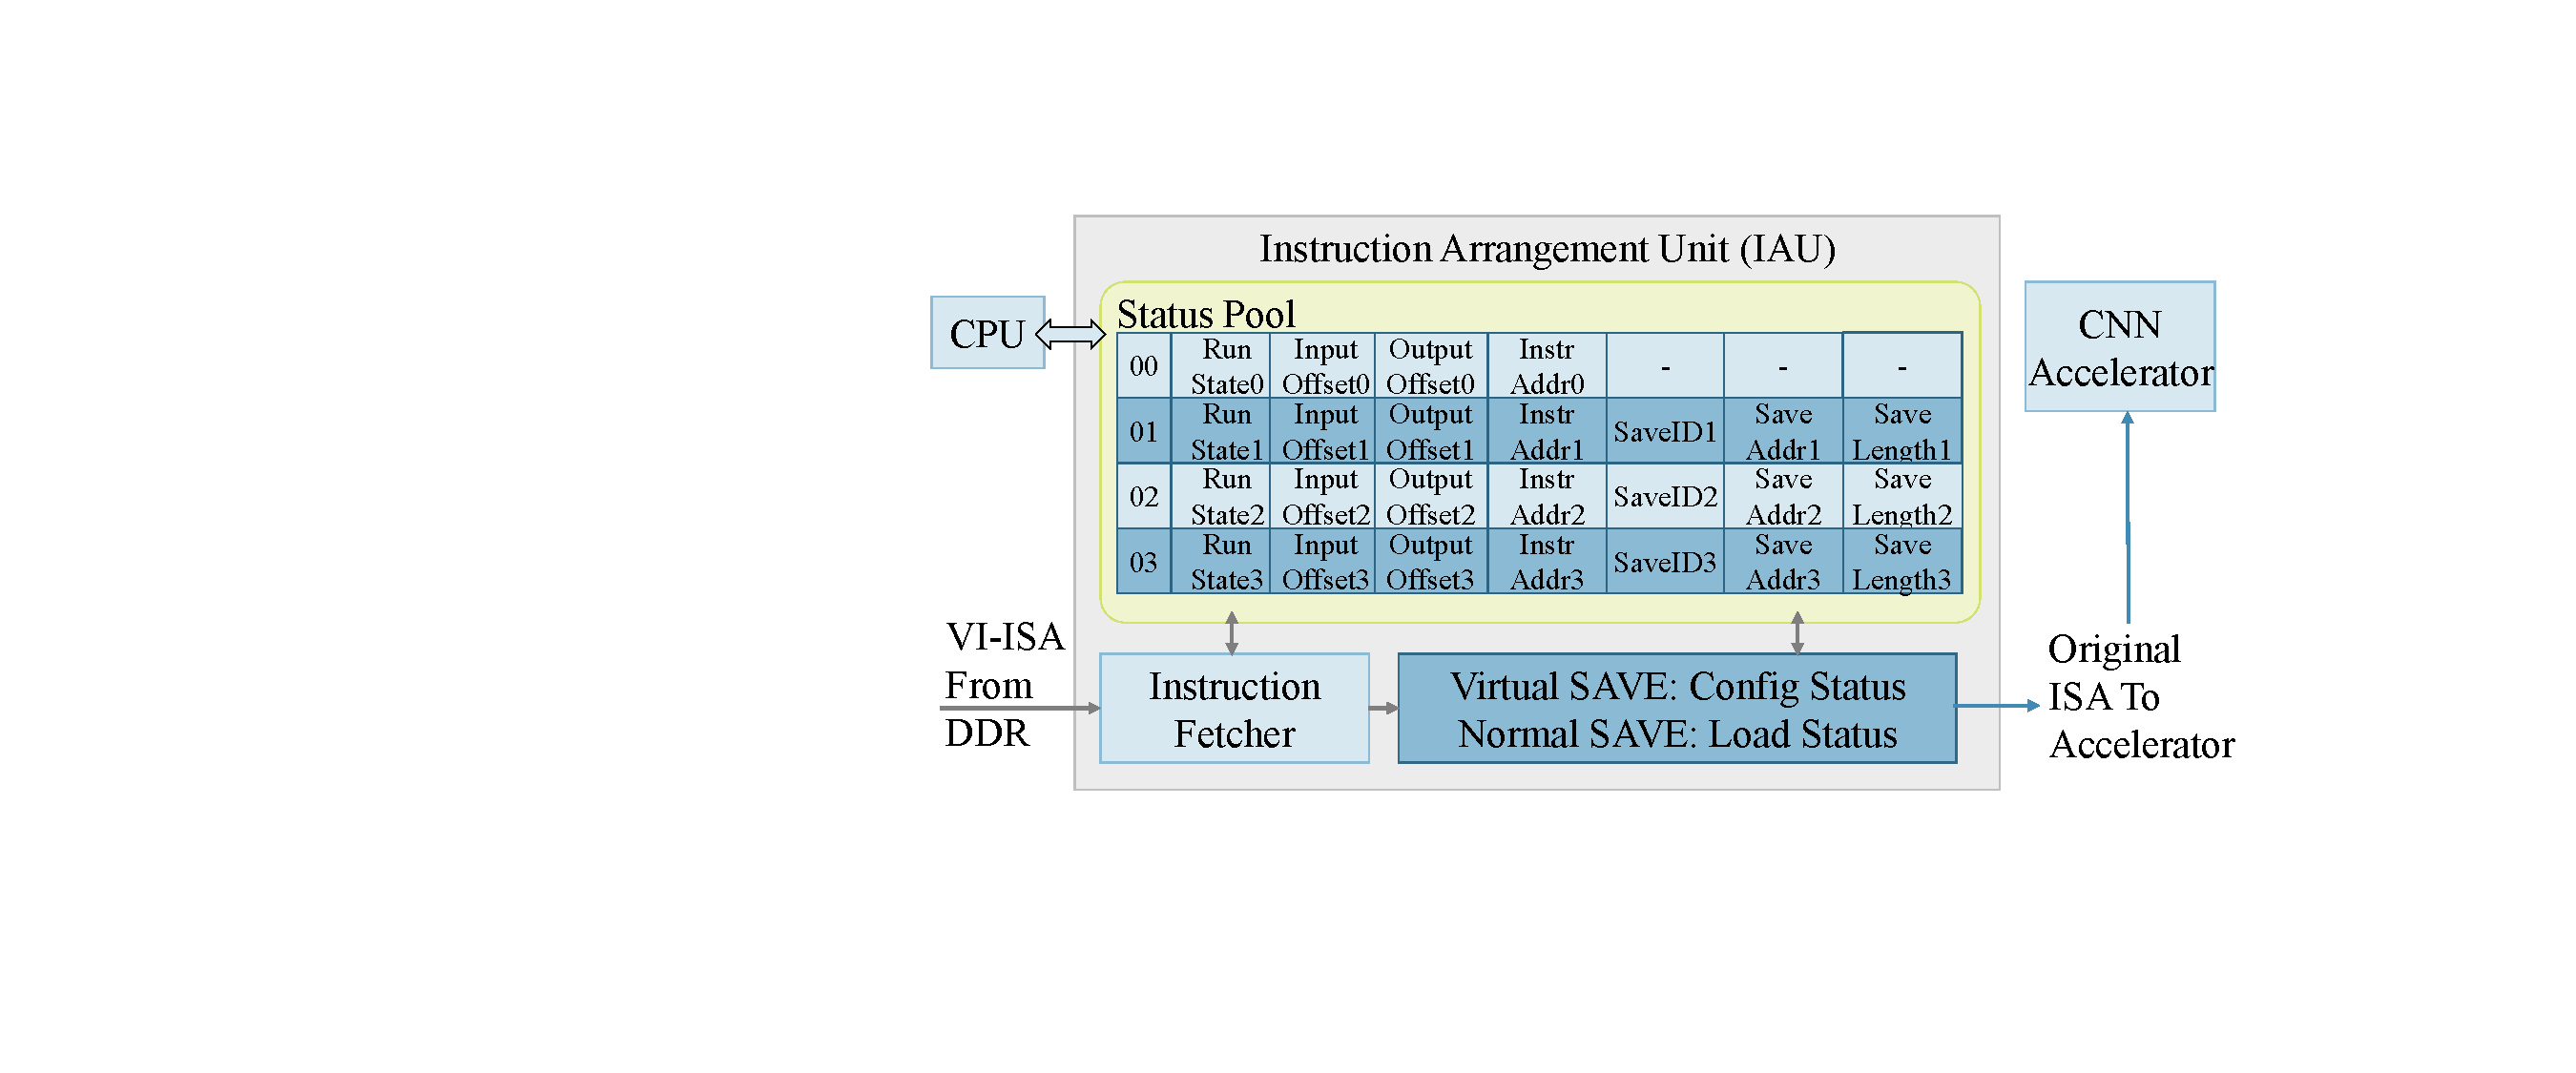
\includegraphics[width=0.99\linewidth]{fig/iau.pdf}
	\vspace{-6mm}
	\caption{Hardware architecture of IAU. The software on the CPU (PS side) communicates with IAU to access the CNN accelerator. IAU records the running state of each task and translates the input instruction virtual instructions sequence (VI-ISA) to a normal sequence of instructions (Original ISA).
	}
	\label{fig:IAU}
\end{figure}

\begin{figure}[t]
	\centering
    % \vspace{-0.1cm} 
    % \setlength{\abovecaptionskip}{0cm} 
    % \setlength{\belowcaptionskip}{-0.4cm} 
	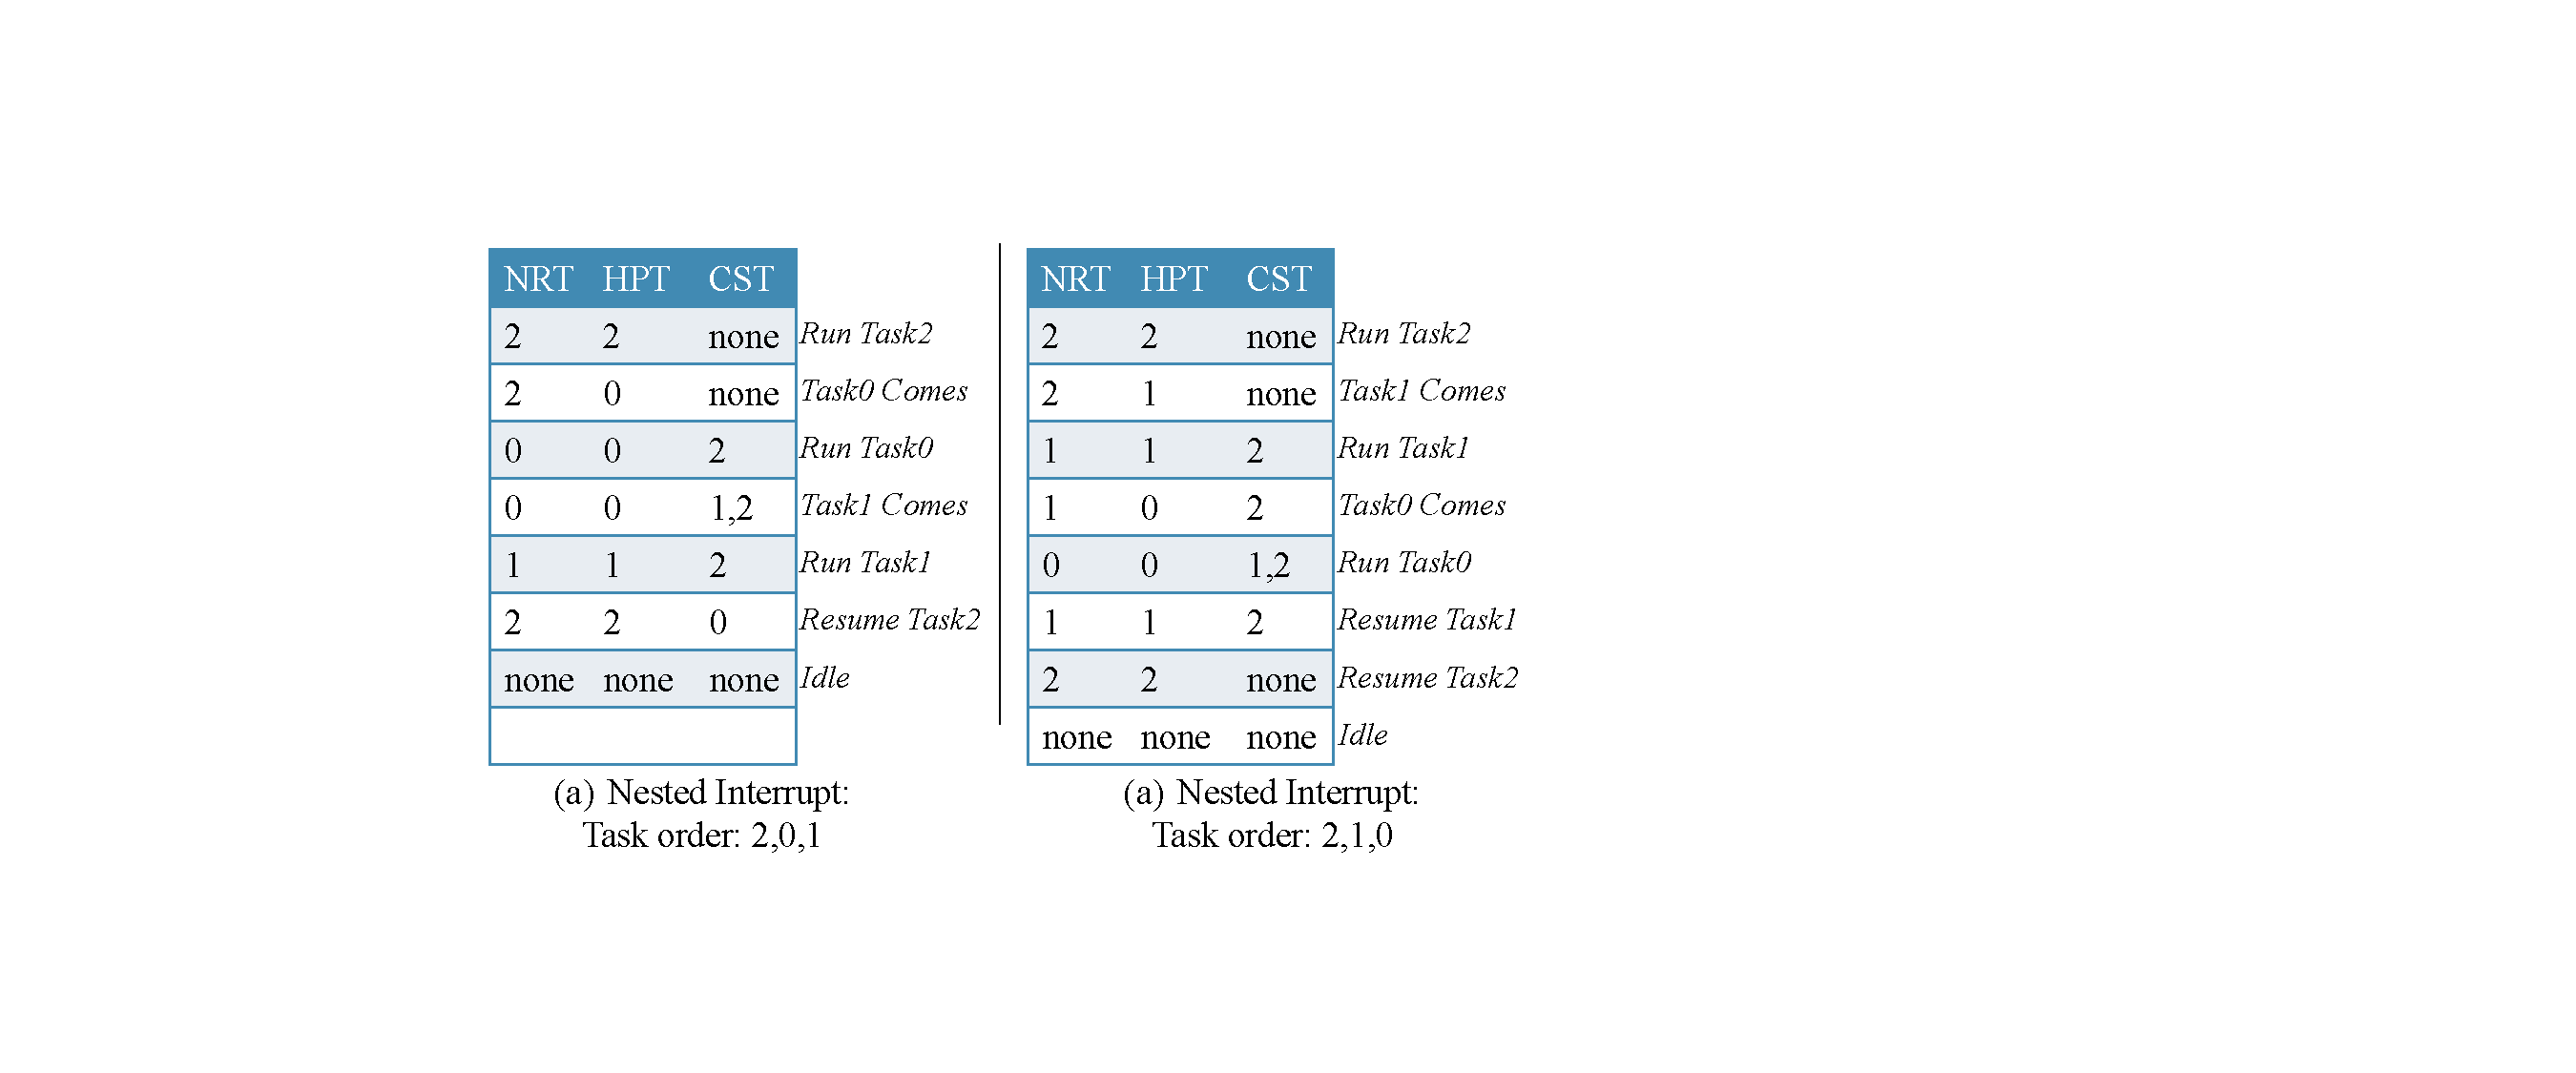
\includegraphics[width=0.8\linewidth]{fig/nestedinter.pdf}
	\vspace{-0mm}
	\caption{
		\textcolor{blue}{The state transition diagram for different task arrangement order.
		}
	}
	\label{fig:nestedinter}
\end{figure}

\begin{figure*}[t]
	\centering
    % \vspace{-0.1cm} 
    % \setlength{\abovecaptionskip}{0cm} 
    % \setlength{\belowcaptionskip}{-0.05cm} 
	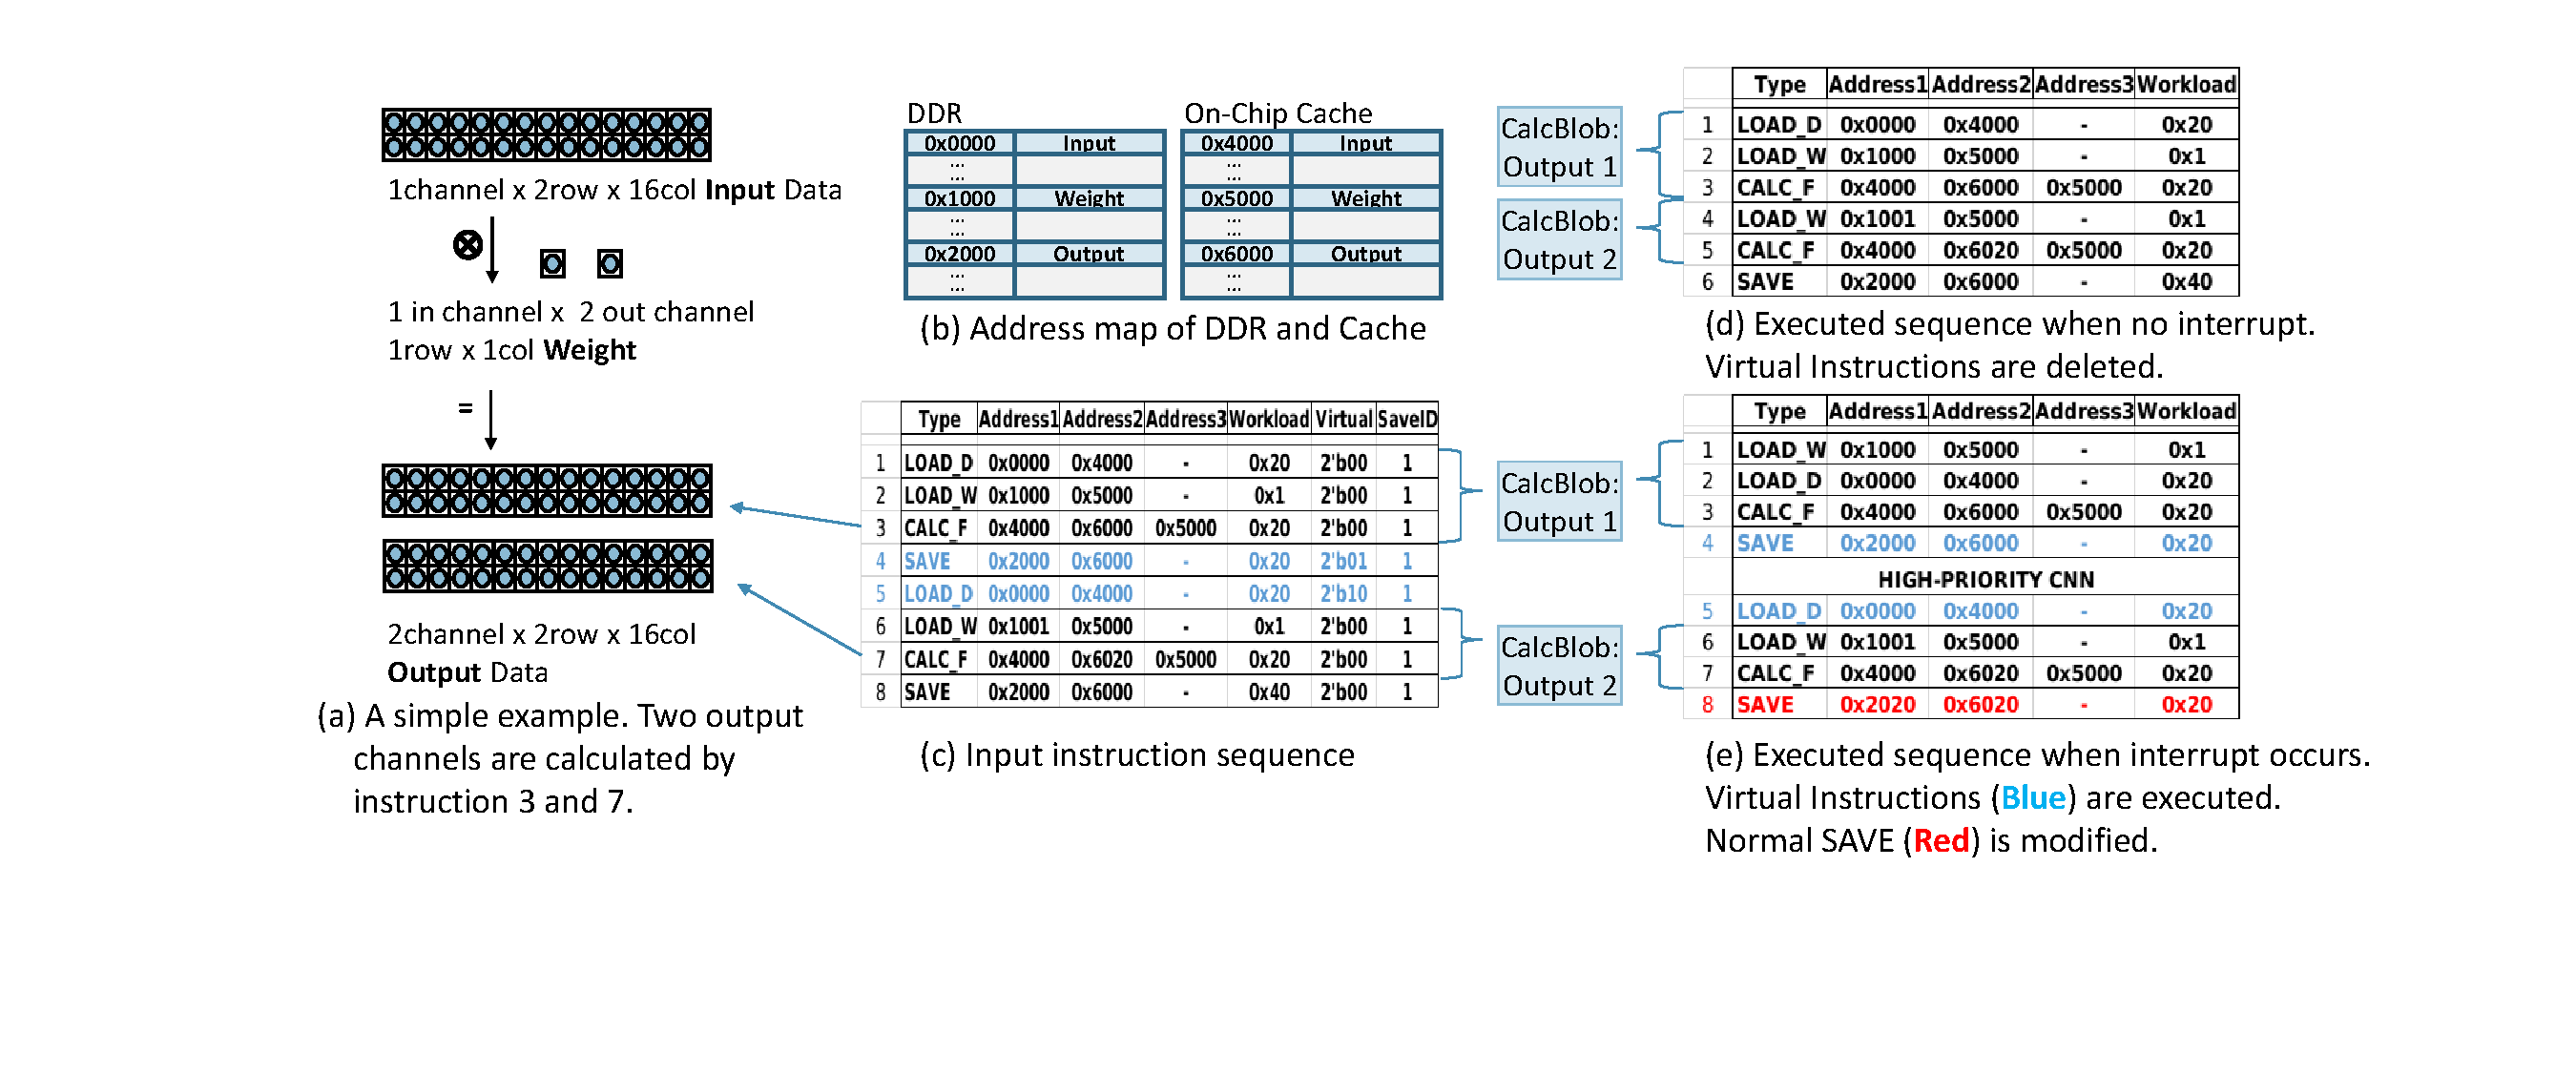
\includegraphics[width=0.9\linewidth]{fig/interexample.pdf}
	\vspace{-5mm}
	\caption{ A simple example of our proposed virtual-instruction-based interrupt. Fig(a), the CNN layer structure. Fig(b), the on-chip and DDR addresses of different data. Fig(c), the instruction sequence in virtual instruction ISA (VI-ISA). The blue instructions are the virtual SAVE and LOAD. Fig(d), executed instructions when no interrupt occurs. Fig(e), executed instructions when an interrupt occurs. }
	\label{fig:interexample}
\end{figure*}


\subsection{ Instruction Arrangement Unit (IAU) }

Instruction Arrangement Unit (IAU) is the hardware to handle the computing requirements of different priority tasks. The IAU monitors the interrupt status and generates the original ISA instruction sequence. The original CNN accelerator does not need to know the interrupt status, and only operates the instructions provided by IAU.

The hardware implementation of IAU is shown in \Cref{fig:IAU}, which supports four tasks with different priorities. Task 0 has the highest priority and is not interruptible. 
InstrAddr records the address to fetch the instructions of the corresponding task. The InputOffset and the OutputOffset, which indicate base address offsets of the input and output data, are configured by the software. 
SaveID, SaveAddr, and SaveLength record the status when an interrupt occurs. 
Subsequent not-virtual SAVE instructions will be modified according to the recorded interrupt status (SaveID, SaveAddr, and SaveLength), to avoid duplicate output data transfer.
% An example of the instruction modification will be given at \Cref{sec:exampleVirtual}.

\textcolor{blue}{
It is easy to support nested interrupt use IAU.
There are three kinds of tasks in IAU, the now-running task (NRT), the highest priority task (HPT), and current stalled tasks (CST).
The state transition of two examples are illustrated in \Cref{fig:nestedinter}.
If $NRT=HPT$, the IAU process normally the task, like "Run Task2" at the beginning of \Cref{fig:nestedinter}(a,b).
If a new high-priority task comes, HPT is set to the high-priority, like "Task 0 Comes" at \Cref{fig:nestedinter}(a). Then, IAU backups the running status of NRT, and store the NRT to CST. And then running the high-priority task, like "Run Task 0" in at \Cref{fig:nestedinter}(a).
If a new task with lower priority than NRT. It is directly stored to CST, like "Task 1 Comes" at \Cref{fig:nestedinter}(a).
When NRT finishes, the highest priority task is poped from CST to run/resume, like "Run Taks1" in \Cref{fig:nestedinter}(a) and "Resume Task2" in \Cref{fig:nestedinter}(b).
In \Cref{fig:IAU}, the IAU can support 4 priorities. 
However, there is only one NN task in each priority. 
If we want to support more priorities, the Instruction Arrangement Unit (IAU) needs more hardware resources to expand Status Pool.
Once the number of max supported priorities is determined and programmed on the hardware, it cannot be modified at runtime.
}


\subsection{Example of Virtual Instruction}
\label{sec:exampleVirtual}


The example is based on a straightforward convolutional layer, which has only one input channel and two output channels. 
The convolution kernel size is $1 \times 1$. The shape of the input and output featuremaps is $ 2 \times 16 $ (\Cref{fig:interexample}(a)). The parallelism of the CALC instruction in this example is $ Para_{in} = 1$ , $ Para_{out}=1$ , $Para_{height}=2$.

Thus, the two output channels are calculated by two CALC\_F instructions (instruction 3 and 7 in \Cref{fig:interexample}(c)). The addresses used in the instruction example are listed in \Cref{fig:interexample}(b). \Cref{fig:interexample}(c) is the instruction sequence from DDR with VI-ISA. \Cref{fig:interexample}(d) is the executed original ISA instructions without interrupt. When an interrupt occurs at the first CalcBlob, \Cref{fig:interexample}(e) illustrates the backup/recovery instructions (Blue) and the modified SAVE instruction (Red). 
% IAU monitors the interrupt status and translates the VI-ISA instruction sequence to the original ISA instruction sequence.

% The hardware implementation of IAU is shouwn in \Cref{{fig:IAU}. There is a Status Pool which records the running states of each task. The InstrAddr is records the instruction address of each CNN